\documentclass{article}
\usepackage{amsmath}
\usepackage{listings}
\usepackage{graphicx}
\usepackage{fullpage}
\title{Latex Exercise}
\date{}
\author{Erik Steenberg}
\begin{document}
\maketitle
\begin{abstract}
Hello. In this report I will explain the exponential function and an approximation of it and test whether or not it will work.
\end{abstract}
\section{Exponential function}
The exponential function, denoted $e^{x}$ or $\exp{x}$ is a function that can be defined as the continous and convergent infinite series,
\begin{equation}\label{eq:exp}
	e^{x}= \sum_0^\infty \frac{x^n}{n!}
\end{equation}
or as the limit
\begin{equation}
	\lim_{n \to \infty} \left(1 + \frac{x}{n}\right)^n
\end{equation}
and is plotted as such,
%\begin{figure}[h]
%	\input{exp.png}
%	\caption{THe exponential function \ref{eq:exp} plotted using the gnuplot in the terminal using makefile.}
%	\label{fig:exp}
%\end{figure}
\\
The exponential function cannot not be below zero. There is of cause eulers function, but that is for another time. 
\\
The exponental function obeys the following relations
\begin{align}\label{eq:rel}
	&\exp(x)*\exp(y) = \exp(x+y)\\
	&\exp(-x)=1/\exp(x)\\
	&\exp(m*x)^n=\exp(n*m*x)\\
\end{align}
The exponentail function is also unique in that it satisfies the diffeneretial equation,
\begin{equation}
	y' = y
\end{equation}
\section{approximation}
In this report, we are to estimate and then check if an approximation, that we have been given, is a good estimation of the exponential function. In c code it is written as, 
\begin{lstlisting}[language=C]
#include<math.h>

double ex(double x){
	if(x<0)return 1/ex(-x);
	if(x>1./8)return pow(ex(x/2),2);
	return 1+x*(1+x/2*(1+x/3*(1+x/4*(1+x/5*(1+x/6*(1+x/7))))));
	}
\end{lstlisting}
Now lets examine the code one line at a time.\\
for the first line, if $(x<0)$ $ex(x)=1/ex(-x)$, now mathematically, this is correct, as we note the relations given in \ref{eq:rel} $\exp(-x)=1/\exp(x)$ which mean that for $x<0$ $\exp(x)=1/\exp(-x)= \exp(-(-x))=\exp(x)$, so for $x<0$ the exponential function is an exponential function. \\
For the second line,  if $(x>1./8)$ $\exp(x) = (\exp(x/2))^2$ again we refer to \ref{eq:rel} $\exp(x)^n=\exp(n*x)$ this means that $(\exp(x/2))^2=\exp(x)$, so for $(x>1./8)$ $\exp(x)=\exp(x)$, like the previous line.\\
For the third line, it returns the first couple of elements in the infinite series representation of the exponential function and should thus also return the exponential function. After all it is often only necessary to include the first couple of terms to get a good representation of the function. So the functions representation of the exponential function also works. So it should work.\\
Plotting the function versus the exponential function from the math header, we get
\begin{figure}[h]
	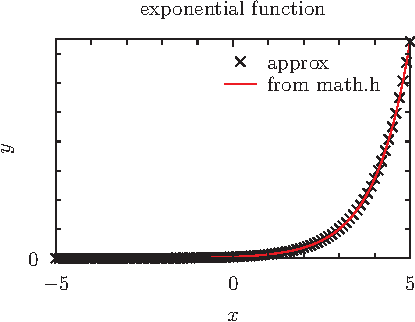
\includegraphics[width=1\textwidth]{pyxplot.pdf}
\end{figure}
We thus conclude that the function is a good approximation. \\
This marks the end of the report.
\end{document}
